% Unofficial University of South Florida (USF) Template.
% A fork of Yale template: https://www.overleaf.com/latex/templates/yale-poster-template/rjpgqfgvsjcv
% which is a fork of the UMich template https://www.overleaf.com/latex/templates/university-of-michigan-umich-poster-template/xpnqzzxwbjzc
% which is fork of the MSU template https://www.overleaf.com/latex/templates/an-unofficial-poster-template-for-michigan-state-university/wnymbgpxnnwd
% which is a fork of https://www.overleaf.com/latex/templates/an-unofficial-poster-template-for-new-york-university/krgqtqmzdqhg
% which is a fork of https://github.com/anishathalye/gemini
% also refer to https://github.com/k4rtik/uchicago-poster



\documentclass[final]{beamer}

% ====================
% Packages
% ====================

\usepackage[T1]{fontenc}
 \usepackage[utf8]{luainputenc}
\usepackage{lmodern}
\usepackage[size=custom, width=122,height=91, scale=1.2]{beamerposter}
\usetheme{gemini}
\usecolortheme{msu}
\usepackage{graphicx}
\usepackage{booktabs}
\usepackage{tikz}
\usepackage{pgfplots}
\pgfplotsset{compat=1.14}
\usepackage{anyfontsize}

%=====================
%Referencias
%====================
% Referencias
\usepackage[
backend=biber,
style=numeric,
sorting=none
]{biblatex}
\addbibresource{Ref Poster MI.bib}

% ====================
% Lengths
% ====================

% If you have N columns, choose \sepwidth and \colwidth such that
% (N+1)*\sepwidth + N*\colwidth = \paperwidth
\newlength{\sepwidth}
\newlength{\colwidth}
\setlength{\sepwidth}{0.025\paperwidth}
\setlength{\colwidth}{0.3\paperwidth}

\newcommand{\separatorcolumn}{\begin{column}{\sepwidth}\end{column}}

% ====================
% Title
% ====================

\title{Inteligencia Artificial en la Medicina. Aplicaciones y dilemas éticos}

\author{Arlet Acosta González}

\institute[shortinst]{Universidad de Salamanca}

% ====================
% Footer (optional)
% ====================

\footercontent{
  \href{https://www.usal.es}{} \hfill
 \hfill
  \href{mailto:  }{}}
% (can be left out to remove footer)

% ====================
% Logo (optional)
% ====================

% use this to include logos on the left and/or right side of the header:
% Left: institution
 \logoright{
\includegraphics[height=8cm]{logo_usal_footer2.png}}

% ====================
% Body
% ====================

\begin{document}



\begin{frame}[t]
\begin{columns}[t]
\separatorcolumn

\begin{column}{\colwidth}

  \begin{block}{Descripción general}

      \begin{figure}
      \centering
                    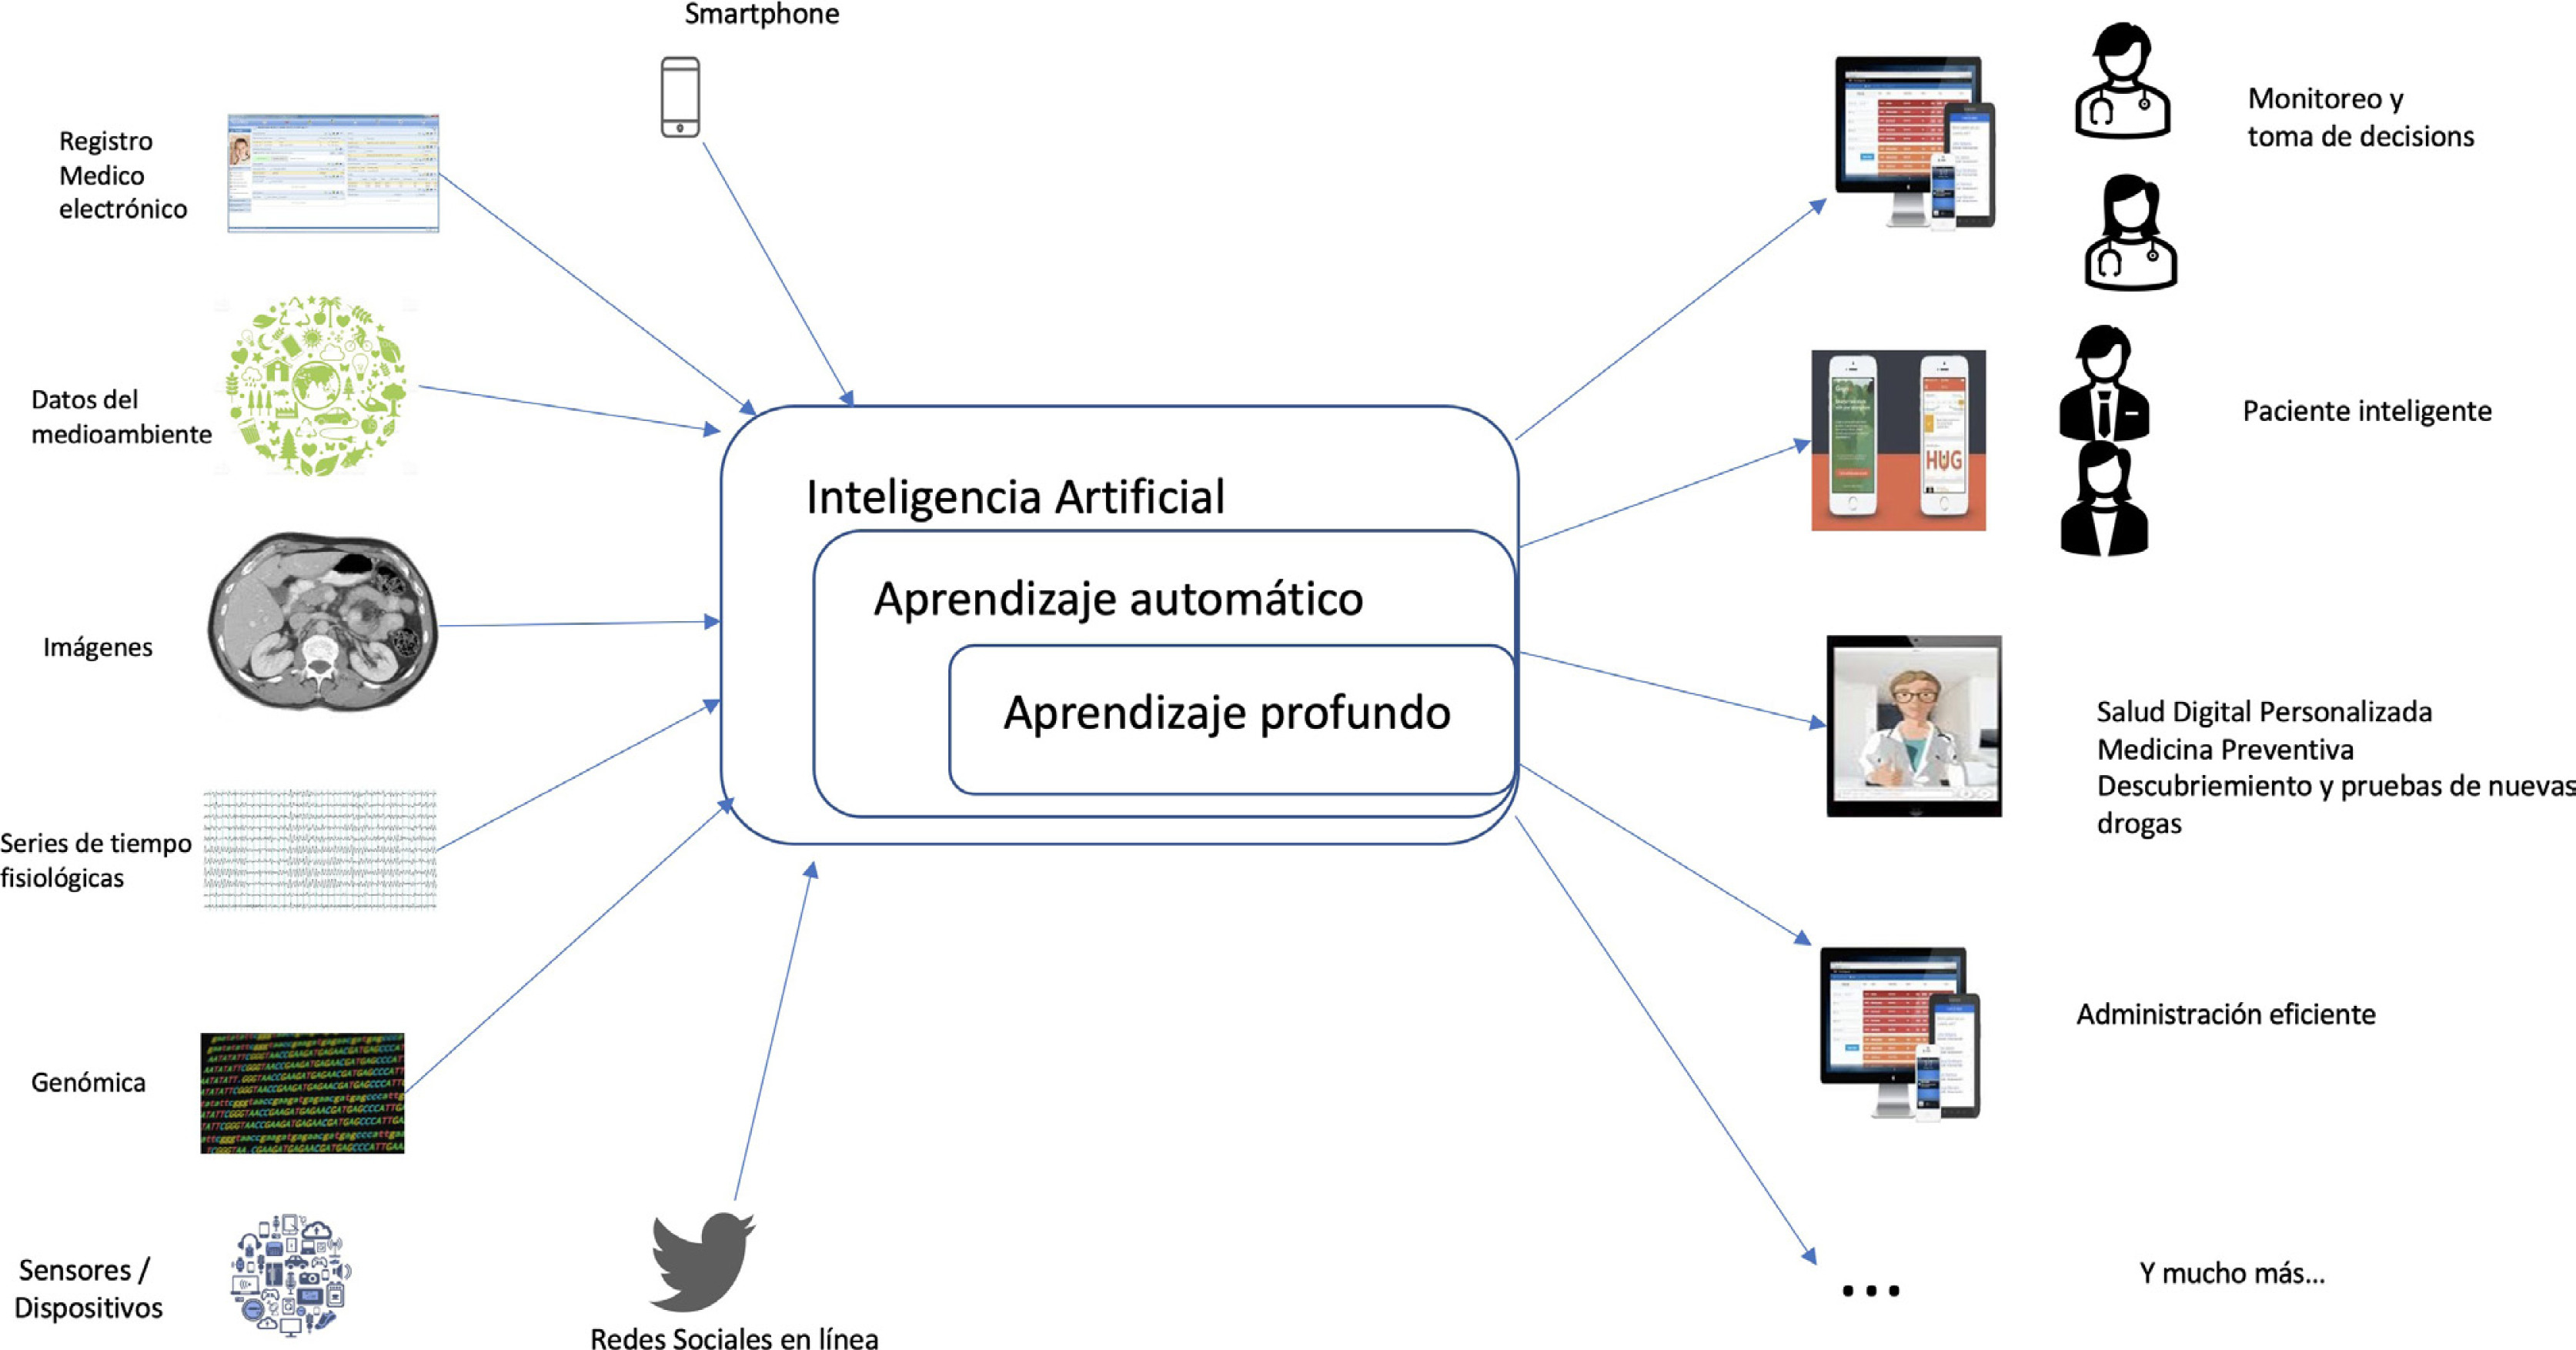
\includegraphics[width=1\textwidth]{high_res.jpg}
    \end{figure}

   La capacidad de los algoritmos de IA para analizar grandes cantidades de datos ha revolucionado la prevención, diagnóstico y tratamiento de diversas enfermedades. Algoritmos informáticos especializados contribuyen a la identificación temprana de enfermedades y la detección de patrones en imágenes médicas, optimizando el proceso de diagnóstico y permitiendo tratamientos más personalizados. 
   
   Sin embargo, este avance no está exento de dilemas éticos. La seguridad de los sistemas, la transparencia en la toma de decisiones y la gestión de datos médicos sensibles son aspectos críticos.\cite{ruiz_inteligencia_2023}

  \end{block}

  \begin{block}{Algunas de las especialidades médicas en las que se aplica IA\cite{lanzagorta-ortega_inteligencia_2023}}

    \begin{itemize}
      \item \textbf{Radiología} 
      \item \textbf{Cardiología} 
      \item \textbf{Neurología} 
      \item \textbf{Oftalmología}
      \item \textbf{Dermatología}
      \item \textbf{Cirugía}

    
    \end{itemize}
    
  \end{block}

  \begin{alertblock}{IA en la Medicina}

    Durante la última década, la investigación de IA aplicada en medicina ha crecido a pasos agigantados. Una de las razones es la gran capacidad de la IA para mejorar la eficiencia y eficacia de la prestación de servicios de salud.

    La IA ha comenzado a incorporarse a la medicina para mejorar la atención al paciente al acelerar los procesos y lograr una mayor precisión diagnóstica, abriendo el camino para brindar una mejor atención médica en general. 

    Sin embargo, no todo es color de rosas. Al tratarse de datos personales sensibles, su tratamiento debe realizarse bajo estrictas medidas de seguridad y consideraciones éticas. 
    


  \end{alertblock}

\end{column}

\separatorcolumn

\begin{column}{\colwidth}

  \begin{block}{Algunos ejemplos del uso de IA en las diferentes áreas de aplicación sanitaria}

    Existen proyectos en la actualidad dedicados a explorar las aplicaciones de la IA en todas las facetas sanitarias: asistencial, diagnóstico, tratamiento y seguimiento de pacientes. A continuación, se comentan algunos ejemplos de las diferentes áreas de aplicación sanitaria.
    
    \begin{enumerate}
      \item \textbf{Asistencial:} Prevención de enfermedades y diagnóstico precoz: Algoritmos para prevenir cáncer de cérvix, identificación de virus del papiloma humano, diagnóstico precoz de cáncer de útero, cabeza, cuello, próstata y piel.      
      \item \textbf{Diagnóstico:}	Software de apoyo al diagnóstico, como Face2Gene® para enfermedades raras, algoritmos de interpretación de imágenes para mejorar la precisión diagnóstica, incluyendo cáncer de mama.
      \item \textbf{Tratamiento:}	Aplicación de IA en combinación con tecnologías como GPS, sensores corporales, para predecir comportamientos de personas mayores y prever reacciones adversas a tratamientos médicos.
      \item \textbf{Seguimiento y monitorización:} Asistentes robóticos con IA para información, comunicación y acompañamiento, como el robot Pillo.\cite{lanzagorta-ortega_inteligencia_2023}
    \end{enumerate}

  \end{block}

  \begin{block}{Tres principios básicos para conseguir una IA fiable:}
\begin{enumerate}
    \item Asegurarse de que la IA esté centrada en el ser humano: La IA se debe desarrollar, implementar y utilizar con un «propósito ético», fundamentado y que refleje los derechos fundamentales, los valores sociales y los principios éticos de la Beneficencia (hacer el bien), Maleficencia (no hacer daño), Autonomía de los seres humanos, Justicia y Explicabilidad.
    \item Confiar en los derechos fundamentales, principios éticos y valores para evaluar prospectivamente los posibles efectos de la IA en los seres humanos y el bien común. Prestar especial atención a las situaciones que involucran a los grupos más vulnerables, como niños, personas con discapacidades o minorías, o situaciones con asimetrías de poder o información, como entre empleadores y empleados, o empresas y consumidores.
    \item Reconocer y tener en cuenta el hecho de que, si bien aporta beneficios sustanciales a los individuos y a la sociedad, la IA también puede tener un impacto negativo. Permanecer atento a las áreas de preocupación crítica.\cite{avila-tomas_inteligencia_2021}
\end{enumerate}

  \end{block}

  \begin{exampleblock}{Recomendaciones del High-Level Expert Group on Artificial Intelligence. Draft Ethics Guidelines for Trust- worthy AI. European Commission\cite{avila-tomas_inteligencia_2021}}
\begin{itemize}
    \item Incorporar los requisitos para la IA de confianza desde la    primera fase de diseño.
    \item Considerar métodos técnicos y no técnicos para garantizar la implementación de esos requisitos en el sistema de IA. Además, tener en cuenta esos requisitos para construir el equipo, para trabajar en el sistema en sí, el entorno de prueba y las aplicaciones potenciales del sistema.
    \item Proporcionar de manera clara y proactiva información a las partes interesadas (clientes, empleados, etc.) sobre     las capacidades y limitaciones del sistema de IA, lo que nos permite establecer expectativas realistas. Asegurar la trazabilidad del sistema de IA es clave en este sentido.
   
  
    
\end{itemize}
  
  \end{exampleblock}

\end{column}

\separatorcolumn

\begin{column}{\colwidth}

  \begin{exampleblock}{}

   \begin{itemize}
     \item Hacer que la IA confiable sea parte de la cultura de la organización, y brindar información a las partes interesadas sobre la implementación, el diseño y el uso de los sistemas de IA. La IA confiable también se puede incluir en deontología o códigos de conducta de las organizaciones.
    \item Asegurar la participación e inclusión de las partes interesadas en el diseño y desarrollo del sistema de IA. Además, asegure la diversidad al configurar los equipos que desarrollan, implementan y prueban el producto.
    \item Prever formación y educación y asegurarse de que los directivos, desarrolladores, usuarios y empleadores conozcan y estén capacitados en IA confiable.
    \item Esforzarse por facilitar la auditabilidad de sistemas de IA, particularmente en contextos o situaciones críticas.
    \item Considerar la posible existencia de conflictos entre             diferentes objetivos (la transparencia puede abrir la puerta al mal uso; identificar y corregir sesgos puede   contrastar con las protecciones de privacidad). Comunicar y documentar estas compensaciones.
    \item Fomentar la investigación y la innovación para promover el cumplimiento de los requisitos para la IA   confiable.
   \end{itemize}

  \end{exampleblock}

  \begin{block}{Conclusiones}
	

\begin{itemize}
    \item La IA ha experimentado un crecimiento significativo en la investigación aplicada a la Medicina en la última década, mejorando la eficiencia y eficacia de la prestación de servicios de salud. 
    \item La capacidad de los algoritmos de IA para analizar grandes cantidades de datos ha revolucionado la prevención, diagnóstico y tratamiento de diversas enfermedades, contribuyendo a la identificación temprana y personalizada de condiciones médicas.
    \item A pesar de los avances positivos, el uso de la IA en Medicina plantea desafíos éticos, especialmente en la gestión de datos médicos sensibles, que requieren medidas de seguridad y consideraciones éticas rigurosas.
    \item La Unión Europea ha establecido principios para guiar el desarrollo ético de la IA en Medicina, enfocándose en centrar la IA en el ser humano, garantizar valores éticos y abogar por la privacidad y la equidad.
\end{itemize}
  
  \end{block}

  \begin{block}{Referencias}

    \nocite{*}
    \footnotesize{\bibliographystyle{plain}\bibliography{}}
    \printbibliography
    

  \end{block}

\end{column}

\separatorcolumn
\end{columns}
\end{frame}

\end{document}
